\begin{figure}[h]\centering\caption{Education Trends, 1996-2011}\begin{tabular}{cc}
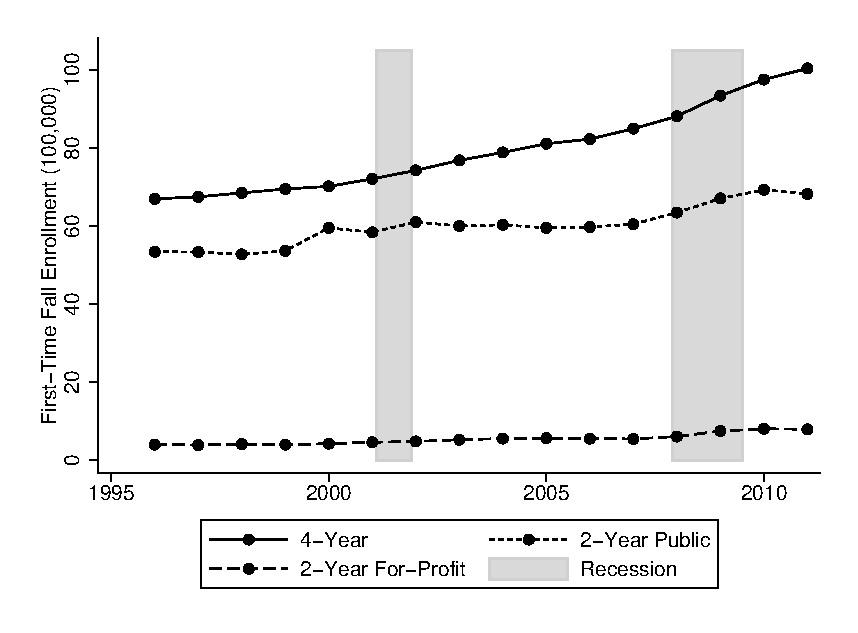
\includegraphics[scale=0.6]{./figures/tef_byyear.eps}&
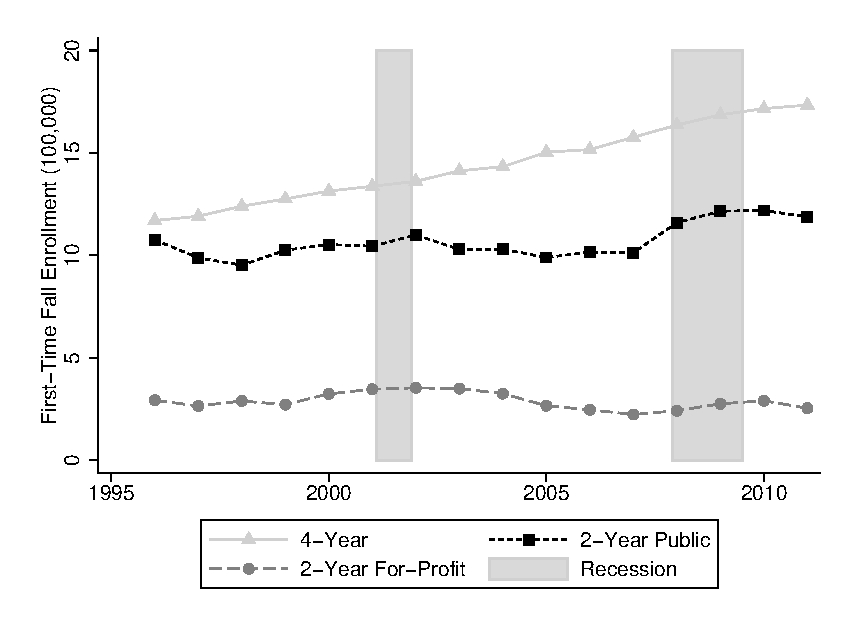
\includegraphics[scale=0.6]{./figures/ffe_byyear.eps}\\
a) Total Enrollment, by Sector&b)First-time Students, by Sector\\

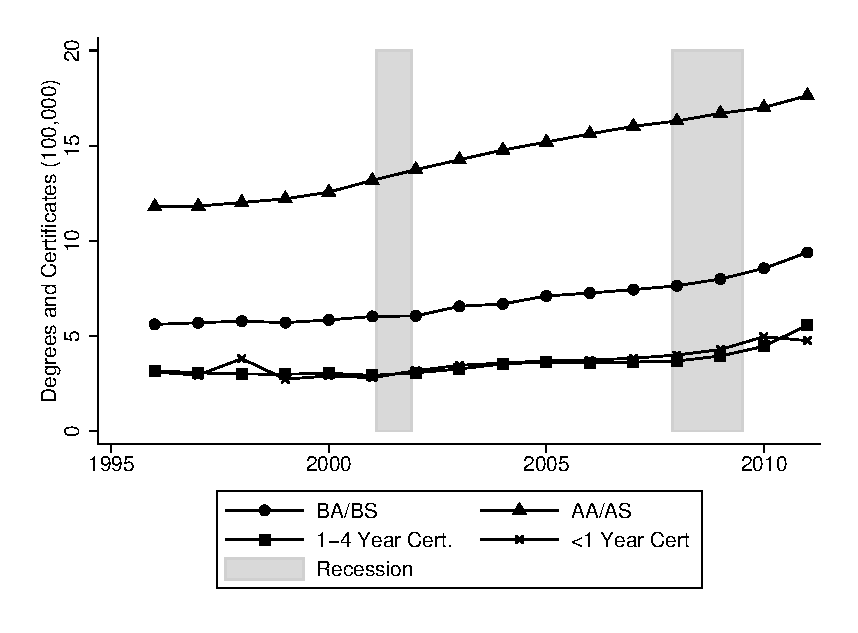
\includegraphics[scale=0.6]{./figures/aw_byyear.eps}&
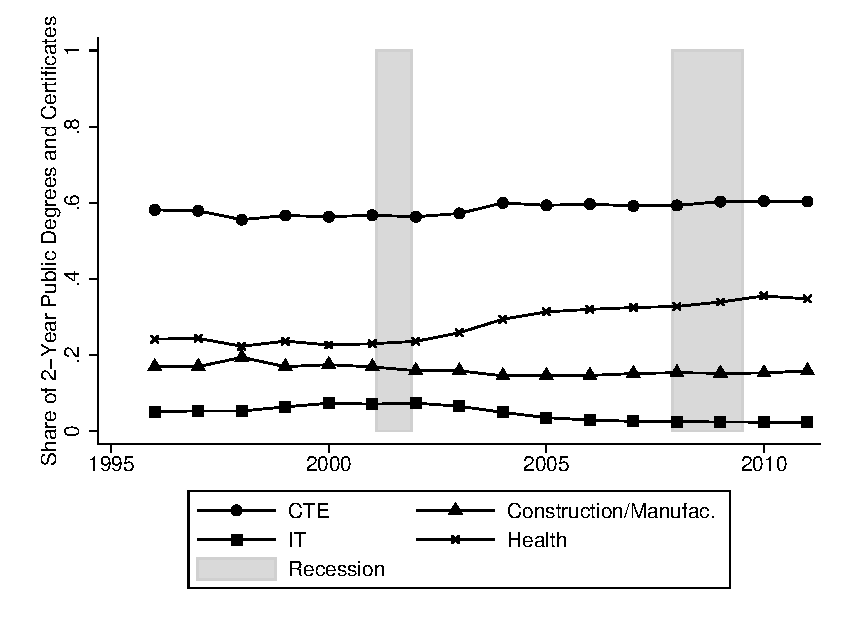
\includegraphics[scale=0.6]{./figures/saw_byyear.eps}\\
c) Total Awards by Type&d) Total 2-Year College Awards by Field\\\\
\multicolumn{2}{p{6in}}{\footnotesize \emph{Notes:} Degree and certificate data is from IPEDS, years 1996-2011. Shaded areas indicate NBER recessions.}
\end{tabular}
\label{fig:grenr}
\end{figure}








\begin{figure}[h]\centering\caption{Enrollment, 2005, Commuting Zones}\begin{tabular}{cc}
\\
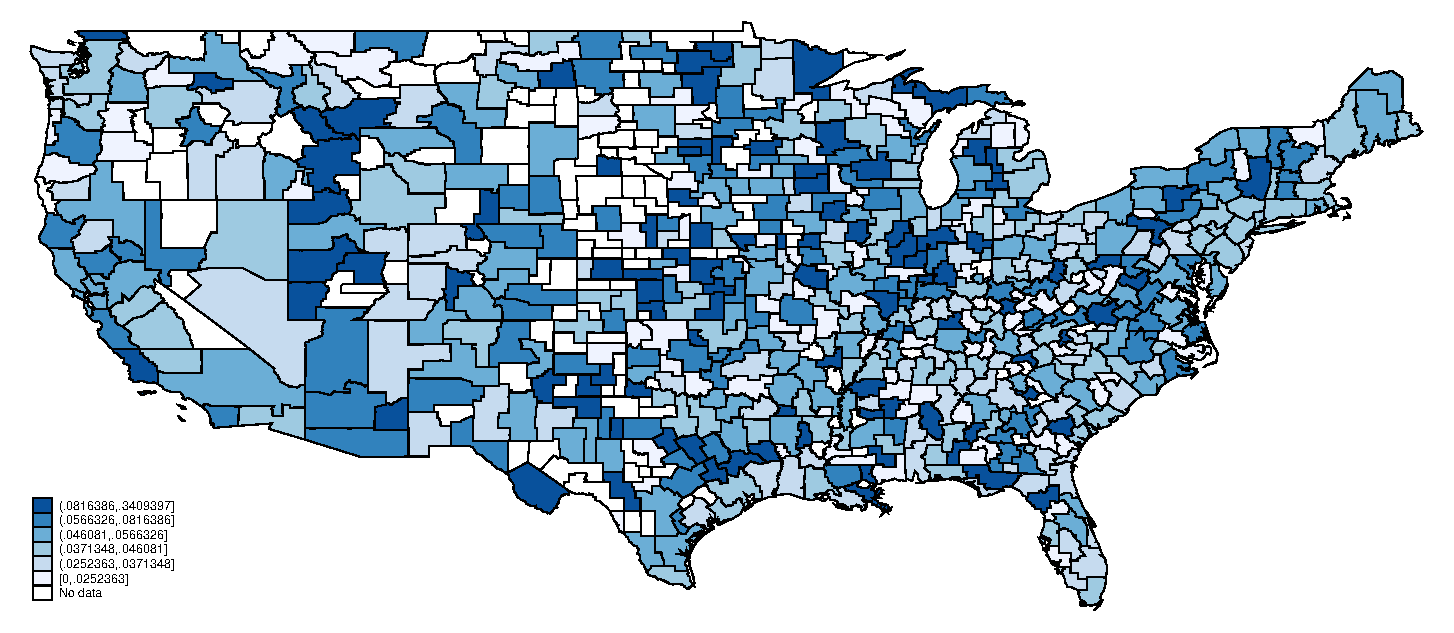
\includegraphics[scale=0.64]{./figures/sh_tef_2005}\\(a) Share of Population in Postsecondary Institutions\\\\
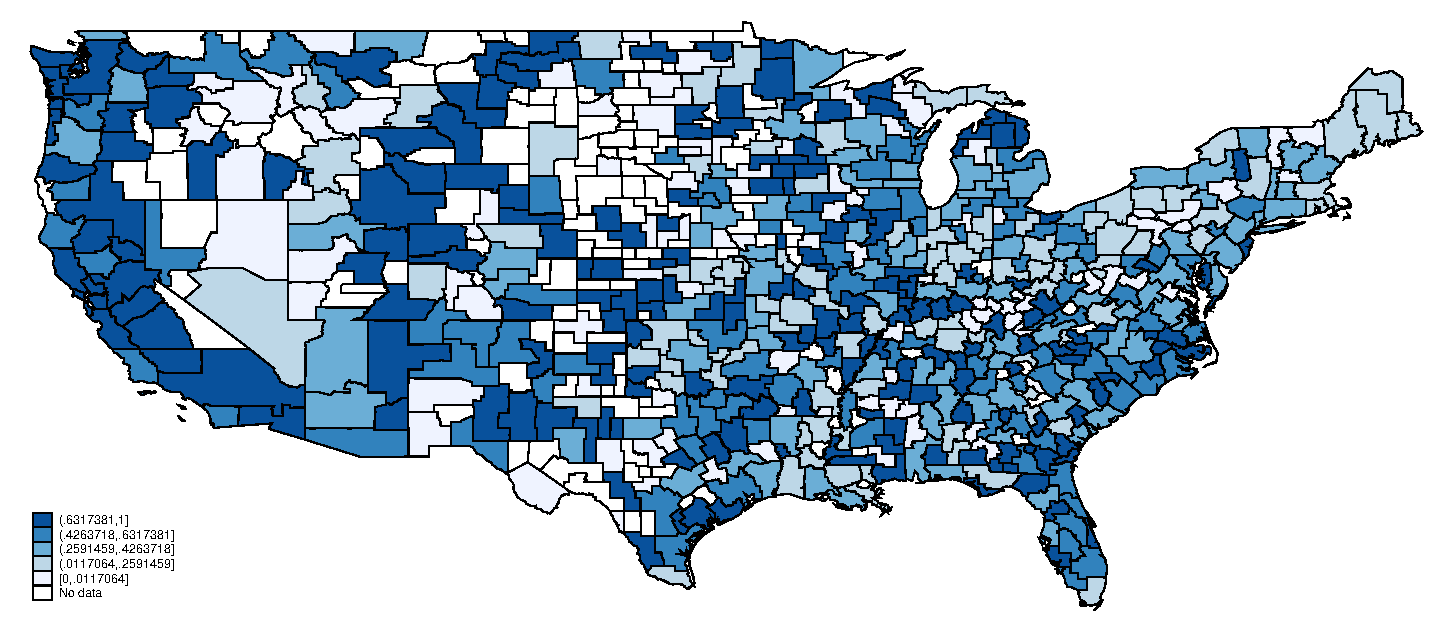
\includegraphics[scale=0.64]{./figures/sh2y_2005}\\
(b) Community College Share of Enrollment\\\\
\multicolumn{2}{p{6in}}{\footnotesize \emph{Notes:} Enrollment data is IPEDS from years 1996-2011, population data is from SEER. Panel (a) displays the share of the population in postsecondary education, while panel (b) displays the share of enrollment accounted for in community colleges.}
\end{tabular}
\label{fig:mapenr}
\end{figure}

\begin{figure}[h]\centering\caption{Content of Community College Awards, 2005, Commuting Zones}\begin{tabular}{cc}
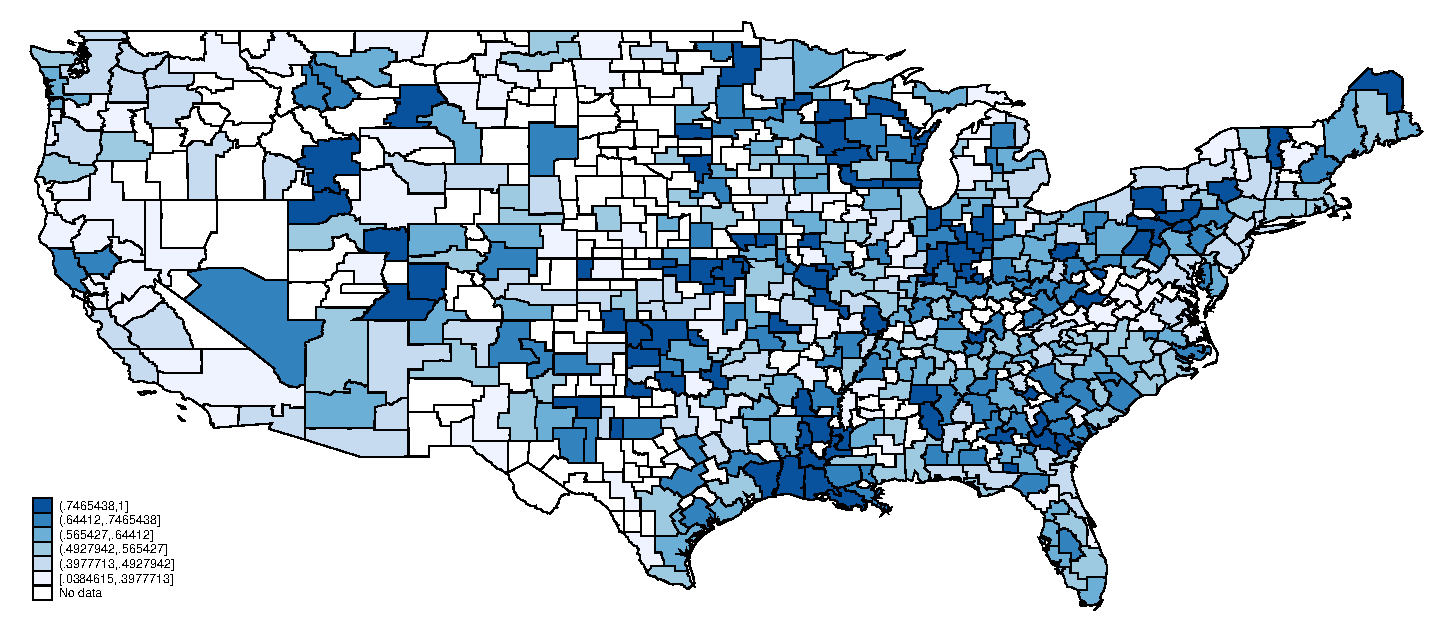
\includegraphics[scale=0.34]{./figures/shaw_CTE_2005}&
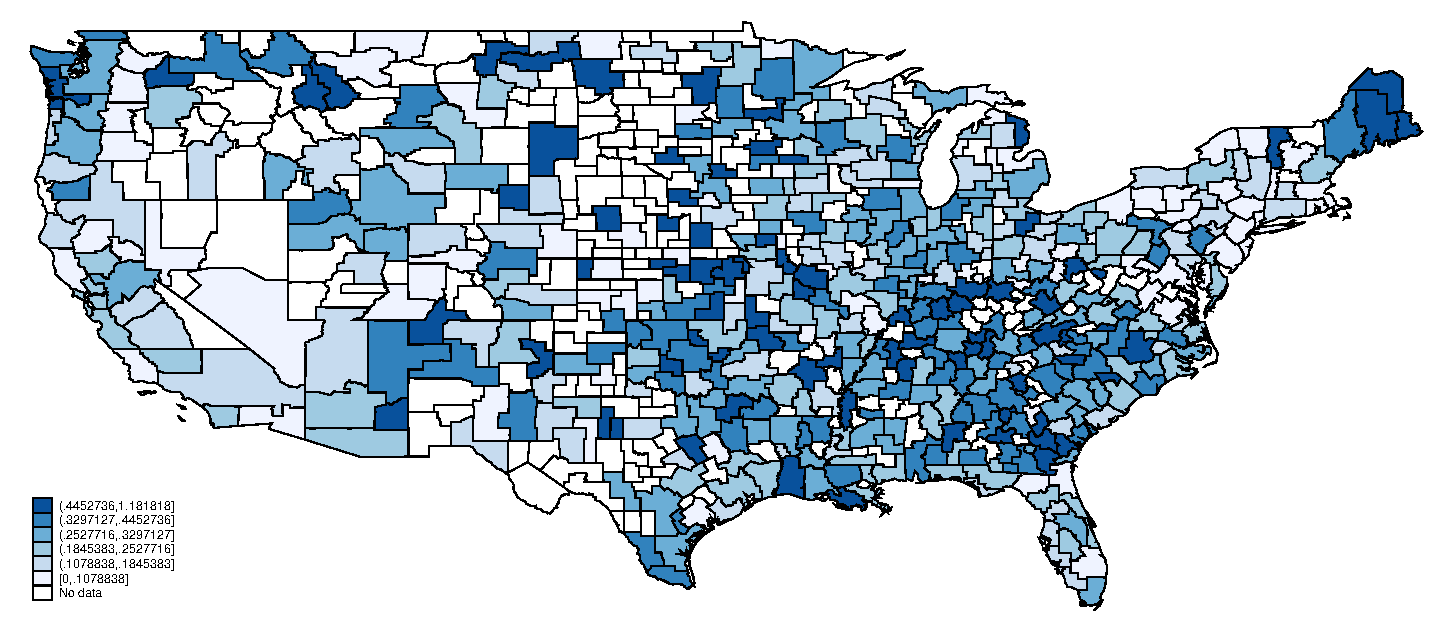
\includegraphics[scale=0.34]{./figures/shaw_CON_2005}\\
(a) Share in CTE&(b) Share in Construction/Manufacturing\\
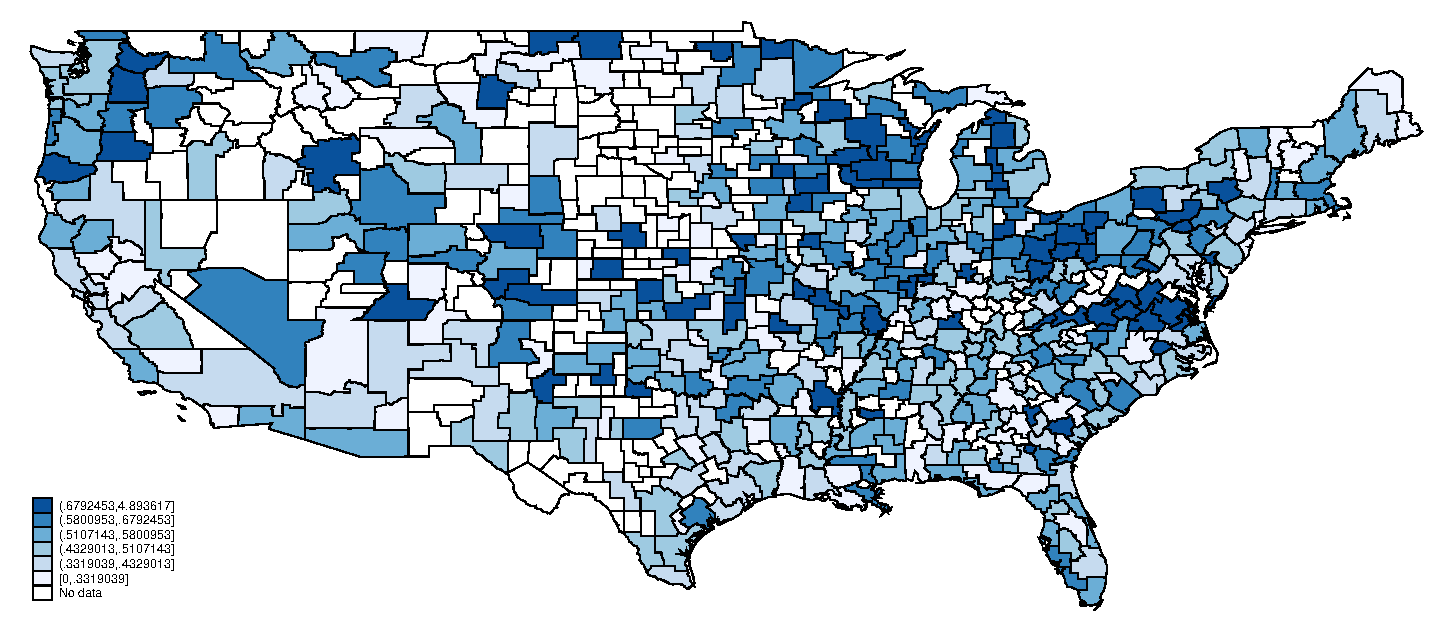
\includegraphics[scale=0.34]{./figures/shaw_HEA_2005}&
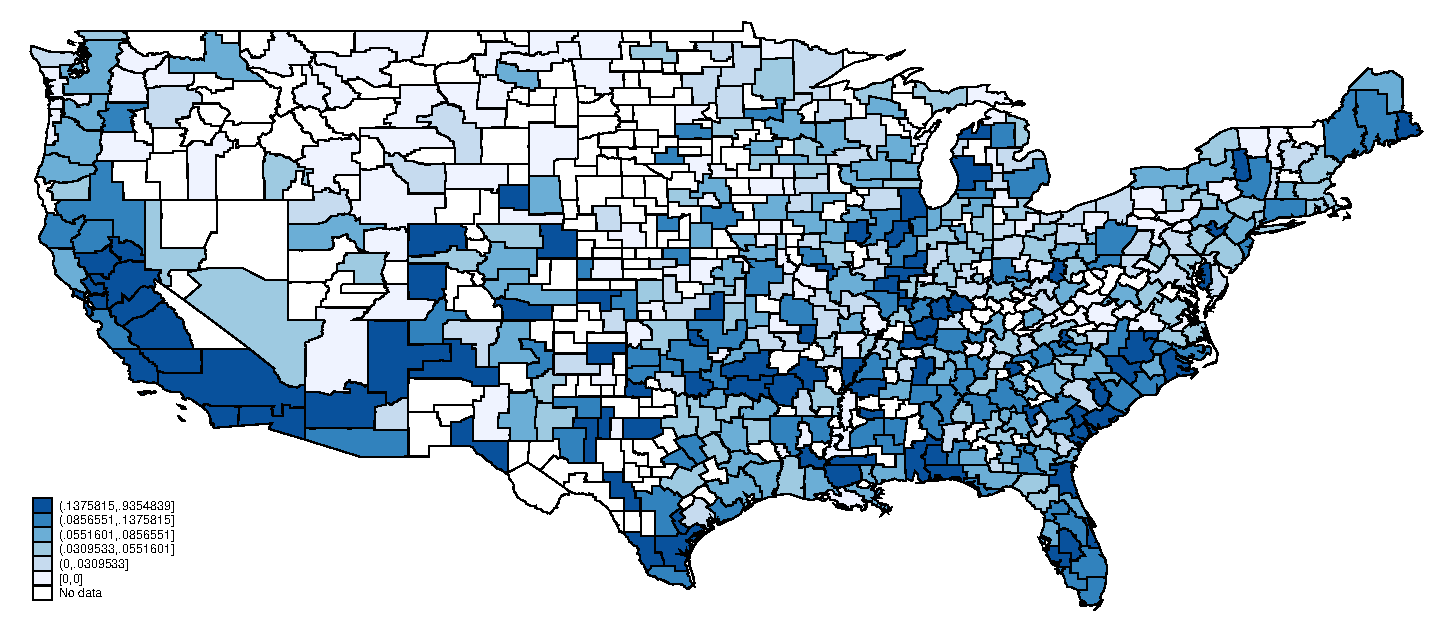
\includegraphics[scale=0.34]{./figures/shaw_FAM_2005}\\
(c) Share in Health&(d) Share in Childcare/Cosmetology\\
\multicolumn{2}{p{\textwidth}}{\footnotesize Notes. Figure (a) shows CTE awards as a share of total awards. Figures  (b)-(d) show awards in the particular field as a share of all CTE awards. }\\
\end{tabular}
\label{fig:mapawa}
\end{figure}




\begin{figure}[h]\centering
\caption{Completion Effects and Estimated Earnings Returns }
\begin{tabular}{cc}
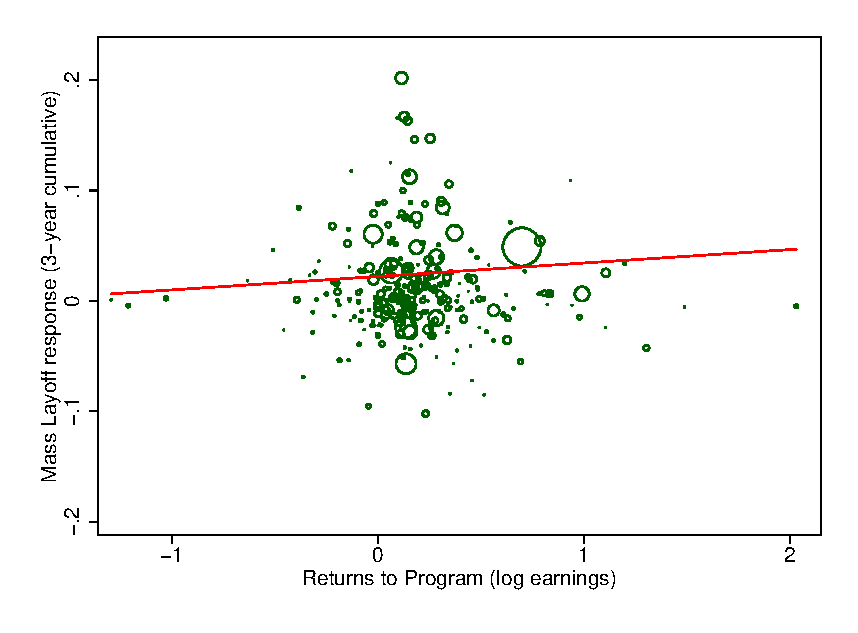
\includegraphics[scale=0.5]{./figures/scatter_bycip_all.eps} &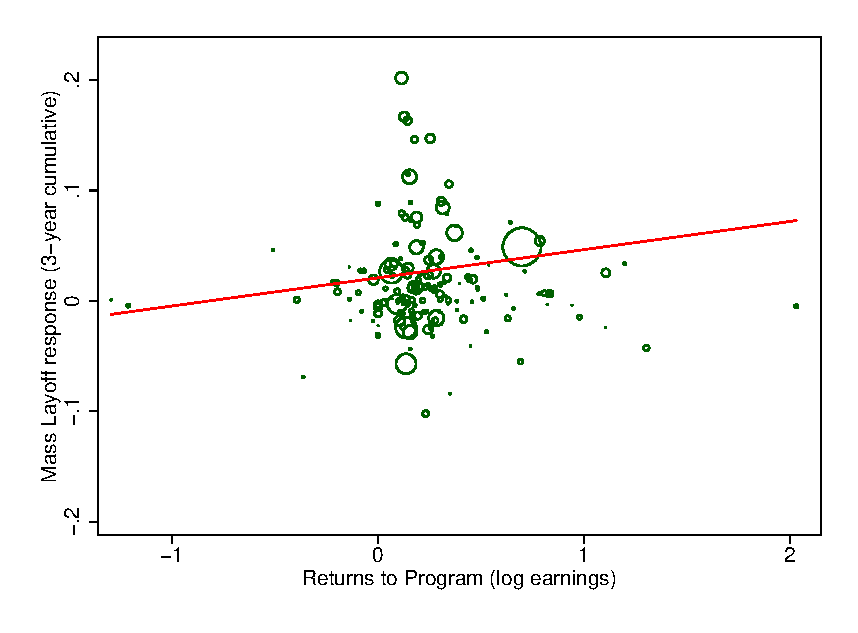
\includegraphics[scale=0.5]{./figures/scatter_bycip_sigret.eps}\\
(a) All Estimates&(b) Statistically Significant Returns Only\\
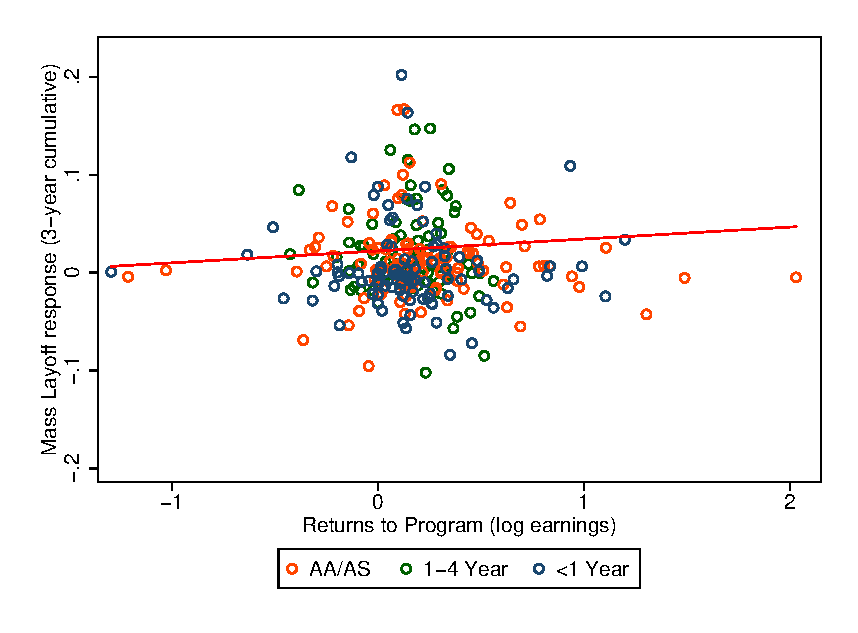
\includegraphics[scale=0.5]{./figures/scatter_bycip_all_bytype.eps} &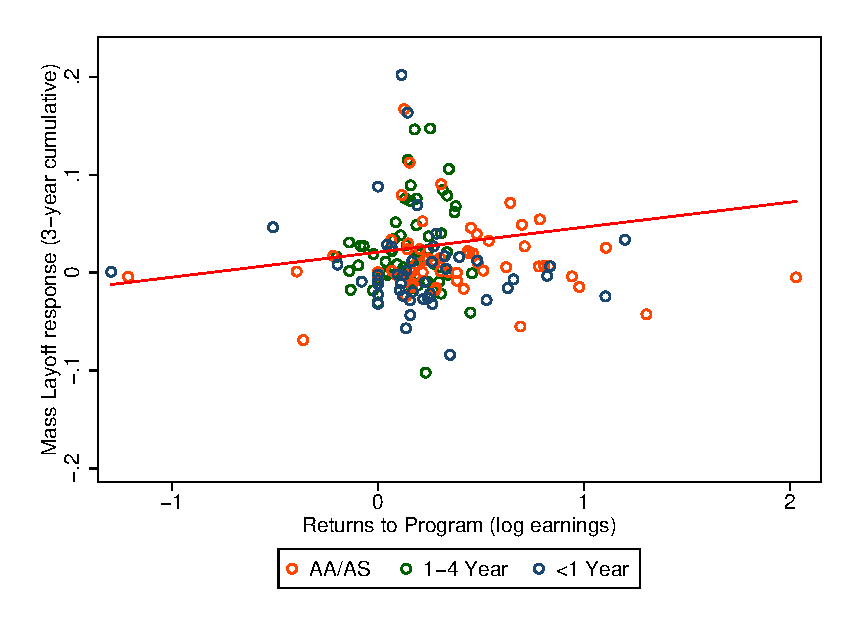
\includegraphics[scale=0.5]{./figures/scatter_bycip_sigret_bytype.eps}\\
(c) All Estimates&(d) Statistically Significant Returns Only\\\\
\multicolumn{2}{p{\textwidth}}{Notes: Estimated returns from \citet{SKG2014} at the 4-digit Taxonomy of Programs level. Regression line, weighted by the average number of graduates of each program each year, is 0.012 (0.01) in panels a) and c) and 0.026 (0.014) in panels b) and d).}\\
\end{tabular}


\label{fig:scatterallsmall}
\end{figure}




\clearpage

\begin{figure}[h]\centering\caption{Impulse Response Function, Community Colleges, Commuting Zones Level}\begin{tabular}{cc}
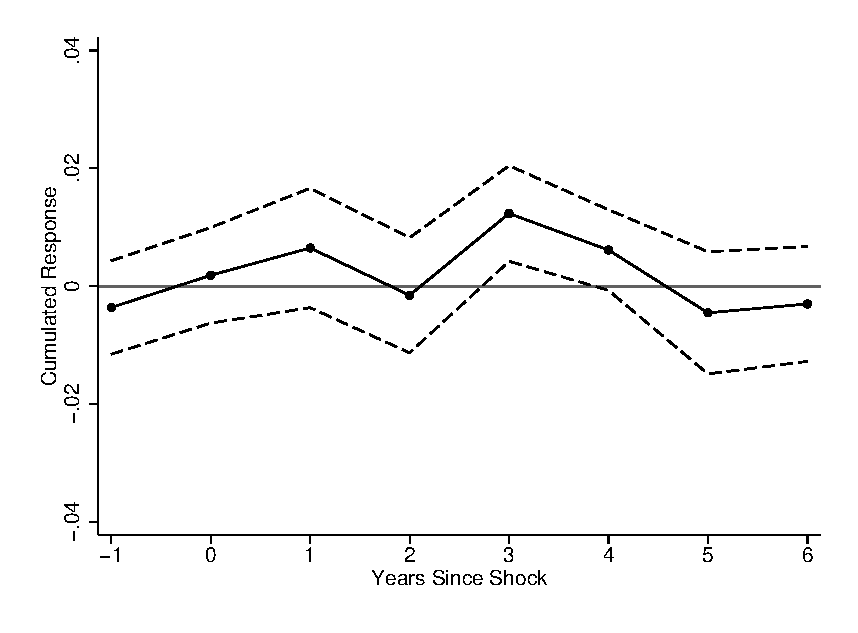
\includegraphics[scale=0.6]{./figures/cumresp_cz_tef_tot47}&
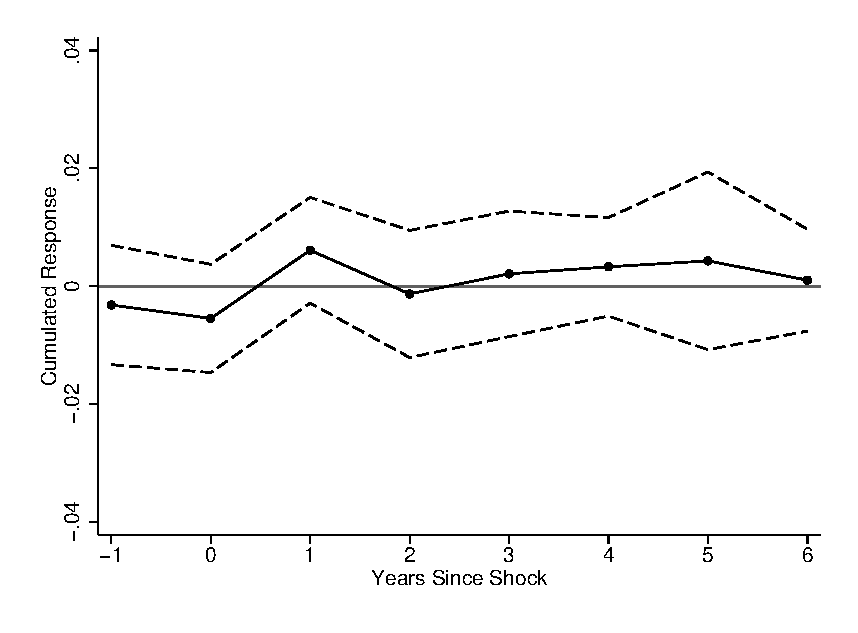
\includegraphics[scale=0.6]{./figures/cumresp_cz_aw_tot47}\\
(a) Fall Enrollment&(b) Total Awards\\
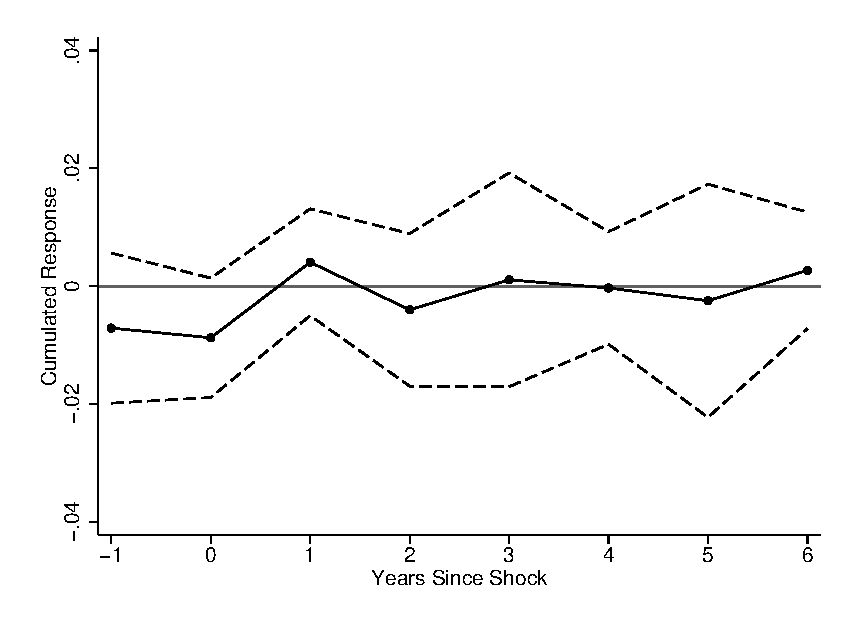
\includegraphics[scale=0.6]{./figures/cumresp_cz_aw_aa47}&
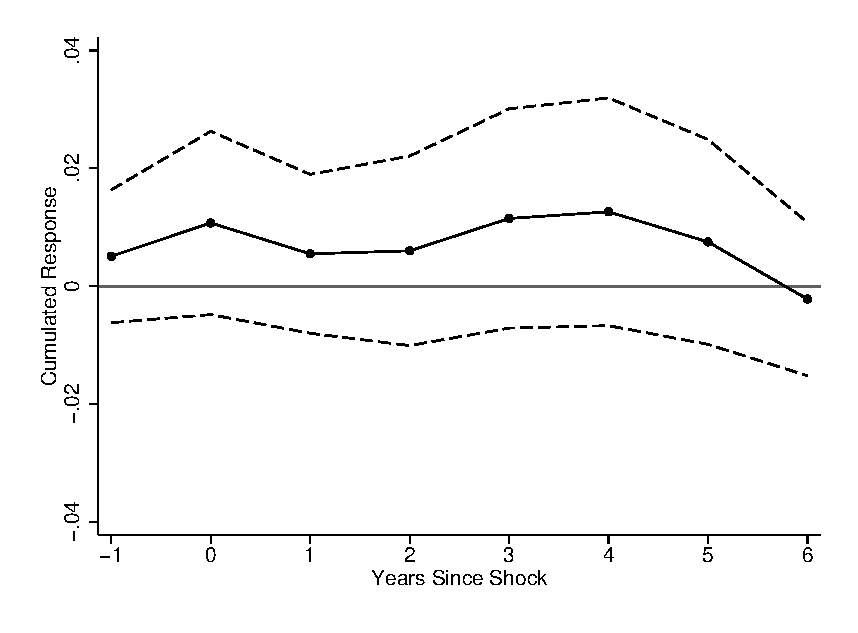
\includegraphics[scale=0.6]{./figures/cumresp_cz_aw_1t447}\\
(c) AA/AS Degrees&(d) 1-4 Year Certificates\\
\multicolumn{2}{p{6in}}{\footnotesize \emph{Notes:} Estimates are from Equation \ref{eqn:localproj}, where the outcome is the panel label. The dotted lines are the 95\% confidence intervals.}
\end{tabular}
\label{fig:czlproj}
\end{figure}



%%%%%%%%%%%%%%%%%%%%%%%%%%%%%%%%%%%%%%%%%%%%%%%%%%%%%%%%%
%Tables
%%%%%%%%%%%%%%%%%%%%%%%%%%%%%%%%%%%%%%%%%%%%%%%%%%%%%%%
\clearpage
\begin{table}[h]\centering\caption{Summary Statistics, 2006-2013}
\def\sym#1{\ifmmode^{#1}\else\(^{#1}\)\fi}\scalebox{0.8}{\begin{tabular}{lc}
\hline\hline

\hline
Workers in Mass Layoffs&   1445.8         \\
                & (6434.5)         \\
Workers in Mass Layoffs as Share of Labor Force&  0.00569         \\
                &(0.00775)         \\
Layoffs $>$ 1\% of Labor Force&    0.203         \\
                &  (0.403)         \\
Layoffs $>$ 5\% of Labor Force&   0.0235         \\
                &  (0.152)         \\
Unemployment Rate&   0.0581         \\
                & (0.0262)         \\
Population (1000s) &    365.7         \\
                & (1047.0)         \\
Population Age 18-60 (1000s) &    206.4         \\
                &  (602.1)         \\
Community Colleges&    2.473         \\
                &  (3.786)         \\
For-Profit 2-year Colleges&    5.294         \\
                &  (16.59)         \\
Community College Fall Enrollment&   9405.8         \\
                &(30857.8)         \\
For-Profit Fall Enrollment&    788.4         \\
                & (2933.5)         \\
No 2-Year Institutions in CZ&   0.0667         \\
                &  (0.250)         \\
Only 2-Year Institutions in CZ&    0.374         \\
                &  (0.484)         \\
Associate's Degrees&   1117.2         \\
                & (2822.0)         \\
1-4 Year Certificates&    559.8         \\
                & (1558.3)         \\
$<$ 1 Year Certificates&    595.8         \\
                & (2027.0)         \\
Share of Awards in CTE&    0.405         \\
                &  (0.174)         \\
Share of Awards in Construction/Manufacturing&   0.0969         \\
                &  (0.110)         \\
Share of Awards in Health&    0.179         \\
                &  (0.118)         \\
Share of Awards in Information Technology&   0.0285         \\
                & (0.0314)         \\
Share of Awards in Public/Protective Services&   0.0380         \\
                & (0.0400)         \\
 
 

\hline\hline
\multicolumn{2}{p{.7\textwidth}}{Notes: Unit of Observation is Commuting Zone by year. Means and standard deviations displayed. }\\
\end{tabular}}
\label{tab:sumstats}
\end{table}







\begin{table}[h]\centering\caption{Mass Layoffs and Two-Year College Enrollment, Degrees and Certificates}
\def\sym#1{\ifmmode^{#1}\else\(^{#1}\)\fi}\scalebox{0.8}{\begin{tabular}{lcccccc}
\hline\hline
&(1)&(2)&(3)&(4)&(5)&(6)\\
&\multicolumn{2}{c}{Fall Enrollment}&\multicolumn{4}{c}{Associate's Degrees and Certificates}\\
&Total&First-Time&Total&AA/AS&1-4 Year Cert& $<$1 Year Cert\\
\hline\\
\multicolumn{4}{l}{\textbf{Community Colleges}}\\
% 
 
Layoffs, t-1    &    0.011         &    0.024\sym{***}&   0.0029         &  -0.0056         &    0.031\sym{*}  &   0.0079         \\
                & (0.0076)         & (0.0092)         & (0.0072)         & (0.0093)         &  (0.017)         &  (0.020)         \\
Layoffs, t-2    &   0.0021         &    0.016\sym{**} &    0.014\sym{**} &   0.0013         &    0.022\sym{**} &    0.038\sym{**} \\
                & (0.0059)         & (0.0071)         & (0.0057)         & (0.0076)         &  (0.011)         &  (0.015)         \\
Layoffs, t-3    &  -0.0017         &   -0.012         &  0.00031         &   -0.018         &    0.022\sym{*}  &    0.012         \\
                & (0.0072)         & (0.0082)         & (0.0054)         &  (0.012)         &  (0.011)         &  (0.015)         \\
 
Total Effect    &    .0111         &    .0287         &     .017         &   -.0227         &    .0741         &    .0584         \\
(se)            &    .0159         &    .0173         &    .0139         &    .0259         &    .0332         &    .0374         \\
P-val           &   0.0000         &   0.0000         &   0.0000         &   0.0000         &   0.0000         &   0.0000         \\
Y-Mean          &  12184.2         &   2138.1         &   1664.7         &   1051.7         &    320.8         &    493.3         \\
Observations    &     6882         &     6882         &     6872         &     6318         &     6714         &     5354         \\
R-sq            &     0.99         &     0.98         &     0.98         &     0.98         &     0.95         &     0.94         \\
 

\\
\hline\\
\multicolumn{4}{l}{\textbf{For-Profits}}\\
% 
 
Layoffs, t-1    &    0.010         &    0.016         &   0.0066         &  -0.0096         &   0.0045         &   0.0045         \\
                & (0.0095)         &  (0.010)         & (0.0085)         &  (0.033)         &  (0.013)         &  (0.021)         \\
Layoffs, t-2    &    0.011         &    0.014         &   0.0071         &   -0.046         &    0.011         &    0.027         \\
                & (0.0088)         & (0.0095)         & (0.0081)         &  (0.029)         &  (0.012)         &  (0.021)         \\
Layoffs, t-3    &    0.012         &    0.011         &    0.025\sym{**} &  -0.0074         &    0.018         &    0.018         \\
                &  (0.011)         &  (0.011)         &  (0.011)         &  (0.033)         &  (0.013)         &  (0.021)         \\
 
Total Effect    &    .0334         &     .041         &    .0386         &   -.0633         &     .034         &    .0499         \\
(se)            &    .0188         &    .0187         &    .0164         &    .0688         &    .0265         &    .0439         \\
P-val           &   0.0000         &   0.0000         &   0.0000         &   0.0000         &   0.0000         &   0.0000         \\
Y-Mean          &   1442.9         &    729.6         &    945.5         &    355.9         &    423.9         &    486.7         \\
Observations    &     4783         &     4783         &     4785         &     2005         &     4656         &     3773         \\
R-sq            &     0.98         &     0.98         &     0.98         &     0.91         &     0.97         &     0.95         \\
 
\\\hline

Year FEs&X&X&X&X&X&X\\
CZ FEs&X&X&X&X&X&X\\
CZ Trends&X&X&X&X&X&X\\
\hline\hline
\multicolumn{7}{p{6in}}{\footnotesize \emph{Notes:} Outcome variables are listed at the top of each column, and are the log counts of the corresponding outcome. Estimates are from equation  \ref{eqn:main}. Panel (a) shows estimates for public community colleges, while panel (b) shows estimates for for-profit schools. All regressions include year and commuting zone fixed effects, commuting zone specific trends. Regressions are weighted by commuting zone population. Standard errors are clustered on commuting zone. *p$<$0.10, ** p$<$0.05, *** p$<$0.01}
\end{tabular}}
\label{tab:main}
\end{table}



\begin{table}[h]\centering\caption{Mass Layoffs and Two-Year College Degrees and Certificates, by Program Type}
\def\sym#1{\ifmmode^{#1}\else\(^{#1}\)\fi}\scalebox{0.8}{\begin{tabular}{lK{2.2cm}K{2.2cm}K{2.2cm}K{2.2cm}K{2.2cm}K{2.2cm}K{2.2cm}}
\hline\hline
&(1)&(2)&(3)&(4)&(5)&(6)&(7)\\
&Total&Career-Technical&Constr./ Manufac.&Health&IT&Public/ Protect.&Childcare/ Cosmet.\\
\hline\\

\multicolumn{6}{l}{\textbf{All Awards}}\\
%\input{../tabfig/lev/reg_mainregawa_ln_aw_tot_47_cz}\hline\\
\multicolumn{6}{l}{\textbf{AA/AS}}\\
%\input{../tabfig/lev/reg_mainregawa_ln_aw_aa_47_cz}\hline\\
\multicolumn{6}{l}{\textbf{1-4 Year Cert}}\\
%\input{../tabfig/lev/reg_mainregawa_ln_aw_1t4_47_cz}\hline\\
\multicolumn{6}{l}{\textbf{$<$1 Year Cert}}\\
%\input{../tabfig/lev/reg_mainregawa_ln_aw_lt1y_47_cz}\\


\hline\hline
\multicolumn{8}{p{7in}}{\footnotesize \emph{Notes:} Estimates are from equation  \ref{eqn:main}. Outcome variables are degrees or certificates awarded in a given field, shown at the column head. Panel (a) shows results for all awards, panel (b) shows results for Associates degrees, panel (c) shows results for longer certificates, and panel (d) shows results for short-term certificate programs. All regressions include year and commuting zone fixed effects, commuting zone specific trends. Regressions are weighted by commuting zone population. Standard errors are clustered on commuting zone. *p$<$0.10, ** p$<$0.05, *** p$<$0.01}
\end{tabular}}
\label{tab:mainbyprog}
\end{table}



\begin{table}[h]\centering\caption{Mass Layoffs and Two-Year College Enrollment, Degrees and Certificates, Before and After 2007}
\def\sym#1{\ifmmode^{#1}\else\(^{#1}\)\fi}\scalebox{0.8}{\begin{tabular}{lcccccc}
\hline\hline
&(1)&(2)&(3)&(4)&(5)&(6)\\
&\multicolumn{2}{c}{Fall Enrollment}&\multicolumn{4}{c}{Degrees and Certificates}\\
&Total&First-Time&Total&AA/AS&1-4 Year Cert& $<$1 Year Cert\\
\hline\\
\multicolumn{4}{l}{\textbf{Community Colleges}}\\
%\input{../tabfig/lev/reg_regprepost_47_cz}
\\
%\hline\\
%\multicolumn{4}{l}{\textbf{For-Profits}}\\
%\input{../tabfig/lev/reg_regprepost_69_cz}\\\hline
Year FEs&X&X&X&X&X&X\\
CZ FEs&X&X&X&X&X&X\\
CZ Trends&X&X&X&X&X&X\\
\hline\hline
\multicolumn{7}{p{6.3in}}{\footnotesize \emph{Notes:} Outcome variables are listed at the top of each column, and are the log counts of the corresponding outcome. Estimates are from equation  \ref{eqn:main}, and allows the effect of mass layoffs to differ before and after 2007. All regressions include year and commuting zone fixed effects, commuting zone specific trends. Regressions are weighted by commuting zone population. Standard errors are clustered on commuting zone. *p$<$0.10, ** p$<$0.05, *** p$<$0.01}
\end{tabular}}
\label{tab:mainrece}
\end{table}



\begin{table}[h]\centering\caption{Mass Layoffs and Two-Year College Enrollment, Degrees and Certificates, Interactions with State-Level Academic Coursework Allowance for UI Beneficiaries}
\def\sym#1{\ifmmode^{#1}\else\(^{#1}\)\fi}\scalebox{0.8}{\begin{tabular}{lccccc}
\hline\hline
&(1)&(2)&(3)&(4)&(5)\\
&\multicolumn{2}{c}{Fall Enrollment}&\multicolumn{3}{c}{Degrees and Certificates}\\
&Total&First-Time&Total&CTE&Academic\\
\hline\\

%\input{../tabfig/lev/reg_reguiaca_47_cz}
\\
%\hline\\
%\multicolumn{4}{l}{\textbf{For-Profits}}\\
%\input{../tabfig/lev/reg_regprepost_69_cz}\\\hline
Year FEs&X&X&X&X&X\\
CZ FEs&X&X&X&X&X\\
CZ Trends&X&X&X&X&X\\
\hline\hline
\multicolumn{6}{p{6.01in}}{\footnotesize \emph{Notes:} Outcome variables are listed at the top of each column, and are the log counts of the corresponding outcome. Estimates are from equation  \ref{eqn:main}, and allows the effect of mass layoffs to differ by whether the state allowed UI beneficiaries to enroll in academic coursework without losing benefits, as in Figure 2 of \citet{BT2015}. All regressions include year and commuting zone fixed effects, commuting zone specific trends. Regressions are weighted by commuting zone population. Standard errors are clustered on commuting zone. *p$<$0.10, ** p$<$0.05, *** p$<$0.01}
\end{tabular}}
\label{tab:mainuibt}
\end{table}





\begin{table}[h]\centering
\caption{Distribution of T-Statistics from Alternate Commuting Zone Definitions}\scalebox{0.8}{
\begin{tabular}{lcccccc}
\hline\hline
&(1)&(2)&(3)&(4)&(5)&(6)\\
&\multicolumn{2}{c}{Fall Enrollment}&\multicolumn{4}{c}{Associate's Degrees and Certificates}\\
&Total&First-Time&Total&AA/AS&1-4 Year Cert& $<$1 Year Cert\\\hline\\
{Layoffs, t-1} &[1.21, 2.20]     & [2.11, 3.06]&[-0.35, 1.11] &[-2.23, -0.45]&[0.967, 1.95]&[0.08, 1.43]\\
{Layoffs, t-2} &[1.14, 2.39]     & [2.91, 4.06] &[1.96, 3.39]&[-0.004, 1.48]&[1.01, 2.57]&[0.94, 2.64]\\
{Layoffs, t-3}& [-1.04, -0.22]     & [-1.82, -0.72] &[-0.29, 1.07]&[-1.53, 0.22]&[1.30, 2.42]&[-0.49, 1.46]\\
\hline\hline
\multicolumn{7}{p{6in}}{\footnotesize \emph{Notes:} Results shown from the test outlined in \citet{FKV2017}, and discussed in Section \ref{sec:robchecks}. The row for each coefficient shows the 2.5th and 97.5th percentile of the distribution of t-statistics on the noted coefficient, when running the analysis with each of  1000 different commuting zone realizations.}
\end{tabular}}
\label{tab:FKVtest}
\end{table}


%
%\begin{table}[h]\centering\caption{Mass Layoffs and Two-Year College Enrollment, Degrees and Certificates, by UI approval}
%\def\sym#1{\ifmmode^{#1}\else\(^{#1}\)\fi}\scalebox{0.8}{\begin{tabular}{lcccccc}
%\hline\hline
%&(1)&(2)&(3)&(4)&(5)&(6)\\
%&\multicolumn{2}{c}{Fall Enrollment}&\multicolumn{4}{c}{Degrees and Certificates}\\
%&Total&First-Time&Total&AA/AS&1-4 Year Cert& $<$1 Year Cert\\
%\hline\\
%\multicolumn{4}{l}{\textbf{Community Colleges}}\\
%\input{../tabfig/lev/reg_reguiaca_47_cz}
%\\
%%\hline\\
%%\multicolumn{4}{l}{\textbf{For-Profits}}\\
%%\input{../tabfig/lev/reg_regprepost_69_cz}\\\hline
%Year FEs&X&X&X&X&X&X\\
%CZ FEs&X&X&X&X&X&X\\
%CZ Trends&X&X&X&X&X&X\\
%\hline\hline
%\end{tabular}}
%\label{tab:mainui}
%\end{table}
